En esta práctica se aborda el problema de localización de un robot móvil. Se considera un robot con un sistema sensor, que tiene un cierto error de medición, y unas balizas, que son los puntos respecto a los que se toman las mediciones. 
En este caso, las balizas son a la vez los objetivos, es decir, describen la ruta que debe seguir el robot. Para esta simulación se calcula la predicción o modelo de la posición del robot, en base al movimiento que se realiza en los actuadores. 
No obstante, este movimiento tiene un cierto ruido, por lo que la posición real del robot dista de la posición ideal o estimada. Por tanto, se deben emplear las mediciones para corregir el modelo y ajustarlo a la realidad.


\section{Código Implementado}
El script proporcionado contiene muchas de las funciones necesarias, sin embargo, se deben implementar código para poder calcular la localización.

\subsection{Análisis}
Se implementan las siguientes características:
\begin{itemize}
  \item \texttt{Función de localización}: Dadas las balizas, el robot ideal, el robot real y las mediciones, se toma un punto de búsqueda a partir del cual se explora un área cuadrada comprendida entre -radio y radio, 
  usando un incremento indicado como parámetro. Se comprueban todas las posiciones posibles dentro de ese área, y se calcula la probabilidad de cada una en función de las mediciones del sensor y las posiciones de las balizas.
  Por último, se devuelve la posición con mayor probabilidad. Esta función se puede observar en la figura \ref{fig:localizacion_fun1}.
  \item \texttt{Localización inicial}: Para comenzar la localización, se debe determinar la posición en la que comienza el robot. \ref{fig:localizacion_inicial}.
  \item \texttt{Ajuste de la posición}: Mientras el robot se mueve, se debe verificar si la posición predicha es correcta, para ello se comprueba la probabilidad de las mediciones de los sensores respecto a la posición predicha.
  Se establece un umbral de error, que al ser superado causa un ajuste de la posición del modelo. Para ello, se emplea la función de localización descrita, tomando un radio de $2*error\_mediciones$. \ref{fig:localizacion_correccion}.
\end{itemize}

En la figura \ref{fig:localizacion_param} se observan algunos de los parámetros que se han indicado del script, más adelante se experimentará con ellos. 

\begin{figure}[htb]
  \centering
  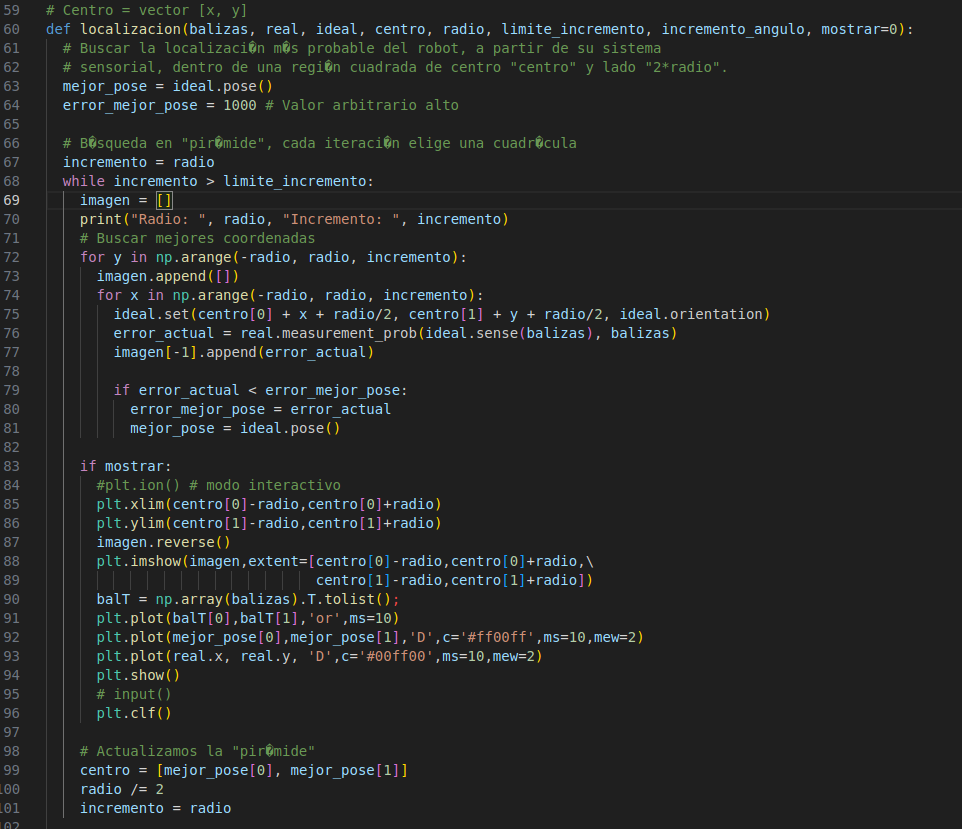
\includegraphics[width=1\linewidth]{images/localizacion1.png}
  \caption{Primera parte de la función de localización}
  \label{fig:localizacion_fun1}
\end{figure}
\begin{figure}[htb]
  \centering
  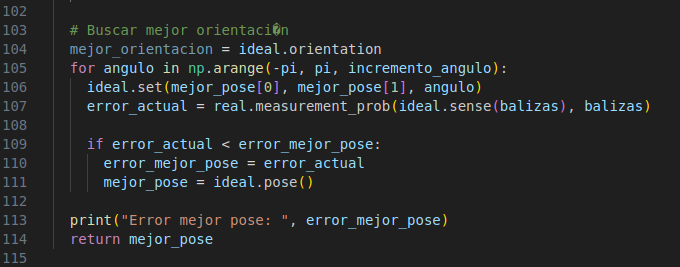
\includegraphics[width=.8\linewidth]{images/localizacion2.png}
  \caption{Fin de la función de localización}
  \label{fig:localizacion_fun2}
\end{figure}
\begin{figure}[htb]
  \centering
  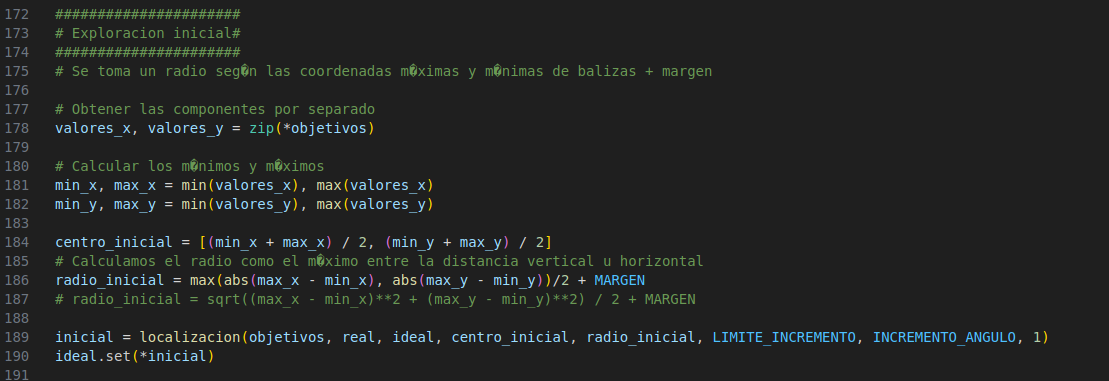
\includegraphics[width=1\linewidth]{images/localizacion5.png}
  \caption{Localización inical}
  \label{fig:localizacion_inicial}
\end{figure}
\begin{figure}[htb]
  \centering
  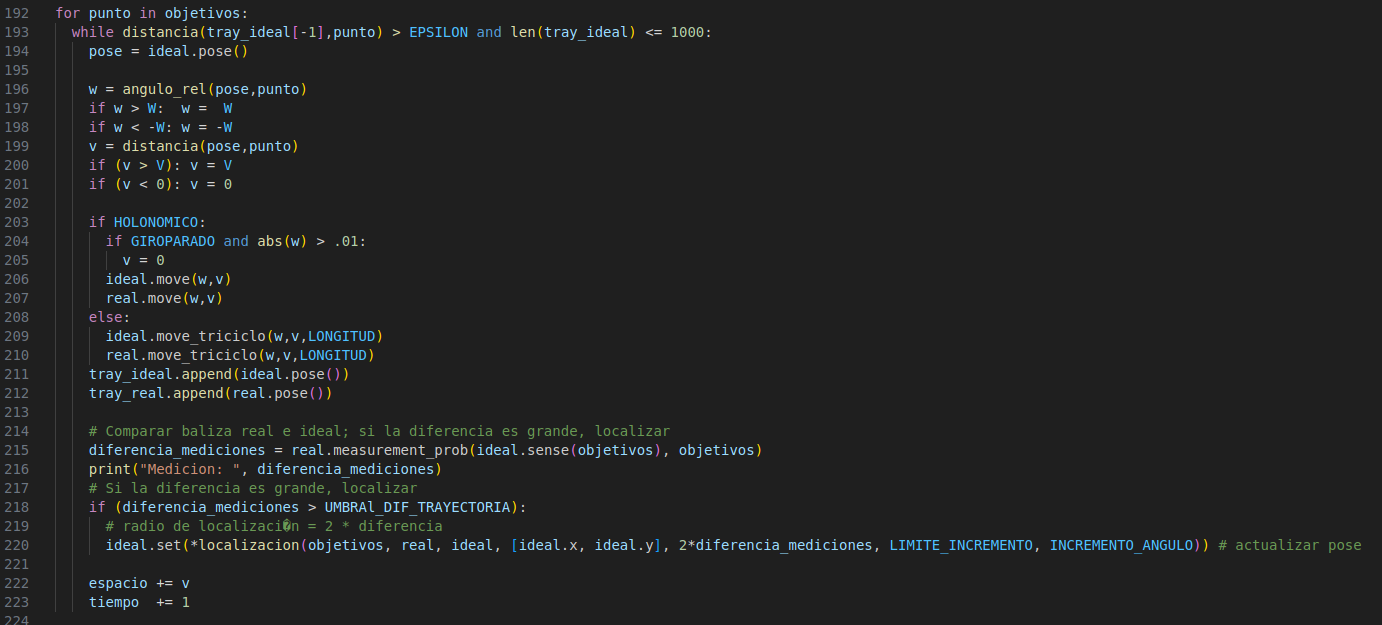
\includegraphics[width=1\linewidth]{images/localizacion6.png}
  \caption{Corrección de la posición}
  \label{fig:localizacion_correccion}
\end{figure}
\begin{figure}[htb]
  \centering
  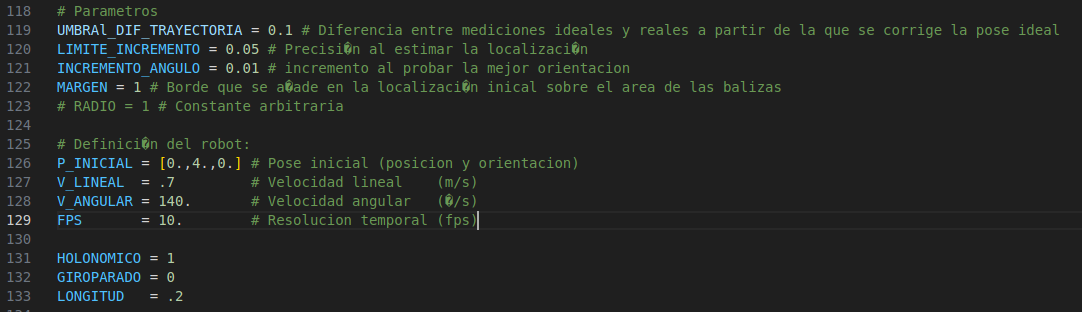
\includegraphics[width=1\linewidth]{images/localizacion3.png}
  \caption{Parámetros de la localización}
  \label{fig:localizacion_param}
\end{figure}

\subsection{Complejidad}
Los cálculos del algoritmo de localización se deben realizar al inicio, y luego cuando se supera el umbral de error. Por tanto, el rendimiento del programa dependerá del ruido en el movimiento, así como del ruido de los sensores, 
y principalmente, del umbral de error considerado. Un mayor umbral resulta en menos cálculos, mientras que un umbral menor requiere una mayor precisión, y por tanto, más cálculos. Se debe tener cuidado, puesto que un umbral demasiado bajo 
puede causar cálculos excesivos debido a los ruidos de sensores.

\bigskip Respecto a la función de localización, su complejidad depende del radio y el incremento considerado. Un menor incremento realiza un barrido más exhaustivo del área, pero requiere más cálculos. Por tanto, es importante elegir un valor que 
consiga un balance entre precisión y rendimiento.

%%%%%%%%%%%%%%%%%%%%%%%%%%%%%%%%%%%%%%%%%%%%%%%%%%%%%%%%%%%%%

\section{Mejoras}

\subsection{Ajuste de la orientación}
\subsection{Uso de incremento piramidal}
\subsection{Cálculo de un radio inicial en función de las balizas y margen}

%%%%%%%%%%%%%%%%%%%%%%%%%%%%%%%%%%%%%%%%%%%%%%%%%%%%%%%%%%%%%
\section{Ejemplos de ejecución}

INCREMENTO 
UMBRAL DE TRAYECTORIA (ERROR)
VELOCIDAD ANGULAR

%%%%%%%%%%%%%%%%%%%%%%%%%%%%%%%%%%%%%%%%%%%%%%%%%%%%%%%%%%%%%
\section{Conclusions}

